\documentclass[tikz,border=10pt]{standalone}
\usetikzlibrary{shapes.geometric, arrows.meta, positioning}
\usepackage{amsmath,amssymb}

\begin{document}
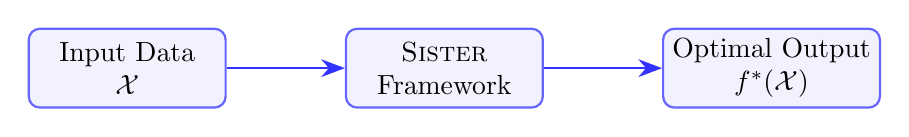
\begin{tikzpicture}[
    box/.style={rectangle, draw=blue!60, fill=blue!5, thick, minimum width=2.5cm, minimum height=1cm, align=center, rounded corners},
    arrow/.style={-{Stealth[length=3mm]}, thick, draw=blue!80}
]

\node (input) [box] {Input Data\\$\mathcal{X}$};
\node (method) [box, right=1.5cm of input] {\textsc{Sister}\\Framework};
\node (output) [box, right=1.5cm of method] {Optimal Output\\$f^*(\mathcal{X})$};

\draw [arrow] (input) -- (method);
\draw [arrow] (method) -- (output);

\end{tikzpicture}
\end{document}
